\documentclass[11pt]{article}

%%%%%%%%%%%%
% Packages %
%%%%%%%%%%%%

\hyphenpenalty=10000
\usepackage{tocloft}
\renewcommand\cftsecleader{\cftdotfill{\cftdotsep}}
\def\undertilde#1{\mathord{\vtop{\ialign{##\crcr
$\hfil\displaystyle{#1}\hfil$\crcr\noalign{\kern1.5pt\nointerlineskip}
$\hfil\tilde{}\hfil$\crcr\noalign{\kern1.5pt}}}}}
\usepackage{cleveref}
\usepackage{xcolor}
\usepackage[colorlinks = true,
            linkcolor = blue,
            urlcolor  = blue,
            citecolor = blue,
            anchorcolor = blue]{hyperref}
\usepackage{epstopdf}
\usepackage{braket}
\usepackage{upgreek}
\usepackage{caption}
\usepackage{booktabs}
\usepackage{subcaption}
\usepackage{amssymb,latexsym,amsmath,gensymb}
\usepackage{latexsym}
\usepackage{graphicx}
\usepackage{float}
\usepackage{enumitem}
\usepackage{pdflscape}
\usepackage{url}
\usepackage{tikz, calc}
\usetikzlibrary{shapes.geometric, arrows, calc}
\tikzstyle{norm} = [rectangle, rounded corners, minimum width=2cm, minimum height=1cm,text centered, draw=black]
\tikzstyle{arrow} = [thick, ->, >=stealth]

\newcommand{\argmin}{\arg\!\min}
\newcommand{\me}{\mathrm{e}}
\providecommand{\e}[1]{\ensuremath{\times 10^{#1}}} 
\providecommand{\mb}[1]{\mathbf{#1}}
\providecommand{\mf}[1]{\mathfrak{#1}}
\providecommand{\ro}[1]{\mathbf{\mathfrak{r}_o}}
\providecommand{\so}[1]{\mathbf{\hat{s}_o}}
\providecommand{\rb}[1]{\mathbf{r_b}}
\providecommand{\rd}[1]{\mathbf{r_d}}
\providecommand{\mh}[1]{\mathbf{\hat{#1}}}
\providecommand{\bs}[1]{\boldsymbol{#1}} 
\providecommand{\intinf}{\int_{-\infty}^{\infty}}
\providecommand{\fig}[4]{
  % filename, width, caption, label
\begin{figure}[h]
 \captionsetup{width=1.0\linewidth}
 \centering
 \includegraphics[width = #2\textwidth]{#1}
 \caption{#3}
 \label{fig:#4}
\end{figure}
}

\newcommand{\tensor}[1]{\overset{\text{\tiny$\leftrightarrow$}}{\mb{#1}}}
\newcommand{\tunderbrace}[2]{\underbrace{#1}_{\textstyle#2}}
\providecommand{\figs}[7]{
  % filename1, filename2, caption1, caption2, label1, label2, shift
\begin{figure}[H]
\centering
\begin{minipage}[b]{.45\textwidth}
  \centering
  \includegraphics[width=1.0\linewidth]{#1}
  \captionsetup{justification=justified, singlelinecheck=true}
  \caption{#3}
  \label{fig:#5}
\end{minipage}
\hspace{2em}
\begin{minipage}[b]{.45\textwidth}
  \centering
  \includegraphics[width=1.0\linewidth]{#2}
  \vspace{#7em}
  \captionsetup{justification=justified}
  \caption{#4}
  \label{fig:#6}
\end{minipage}
\end{figure}
}
\makeatletter

\providecommand{\code}[1]{
\begin{center}
\lstinputlisting{#1}
\end{center}
}

\newcommand{\crefrangeconjunction}{--}
%%%%%%%%%%%
% Spacing %
%%%%%%%%%%%
% Margins
\usepackage[
top    = 1.5cm,
bottom = 1.5cm,
left   = 1.5cm,
right  = 1.5cm]{geometry}

% Indents, paragraph space
%\usepackage{parskip}
\setlength{\parskip}{1.5ex}

% Section spacing
\usepackage{titlesec}
\titlespacing*{\title}
{0pt}{0ex}{0ex}
\titlespacing*{\section}
{0pt}{0ex}{0ex}
\titlespacing*{\subsection}
{0pt}{0ex}{0ex}
\titlespacing*{\subsubsection}
{0pt}{0ex}{0ex}

% Line spacing
\linespread{1.1}

%%%%%%%%%%%%
% Document %
%%%%%%%%%%%%
\begin{document}
\title{\vspace{-2.5em} Spatio-angular Kernels and Transfer Functions for Fluorescence Microscopes \vspace{-2.5em}} \author{Talon Chandler}% and Patrick La Rivi\`ere}
\date{\vspace{-1em}\today\vspace{-1em}}
\maketitle
\section{Introduction}
In these notes we will consider a single-view fluorescence microscope
\textbf{with no polarizing filters} that uses TIRF excitation to excite
fluorophores in all orientations equally. This excitation scheme allows us to
focus exclusively on the detection process. We will find the spatio-angular
kernel of this microscope and analyze it in the frequency domain using the
spatio-angular Fourier transform. Along the way we will show that uniform
excitation fluorescence microscopes have spatial and angular band-limits.

We use plain roman type for scalars, e.g., $x, y, z$; bold lowercase roman type
for two-dimensional vectors, e.g., $\mb{r}$; hats for unit vectors, e.g.,
$\mb{\hat{s}}$; bold lowercase gothic type for three-dimensional vectors, e.g.,
$\mb{\mathfrak{r}}$; and bold capital roman type for matrices, e.g., $\mb{R}$.

\section{General Forward Model}
Consider a three-dimensional field of oriented fluorescent dipoles. We can
represent the entire object using a function $f(\ro{}, \so{})$ that
returns the number of dipoles at position $\ro{}$ per unit volume oriented in
direction $\so{}$ per unit solid angle. 

The intensities measured using a general linear measurement system can by
modeled using
\begin{align}
  g_i(\rd{}) = \int_{\mathbb{R}^3}d\ro{} \int_{\mathbb{S}^2}d\so{}\ h_i(\rd{}; \ro{}, \so{})f(\ro{}, \so{})
\end{align}
where $g_i(\mb{r_d})$ is the camera frame collected under the $i$th measurement
configuration ($i$ indexes polarizer settings or views), $\mb{r_d}$ is the
two-dimensional detector coordinate, and
$h_i(\rd{}; \ro{}, \so{})$ is the spatio-angular kernel of the
$i$th measurement configuration. Our goal is to reconstruct the object
$f(\ro{}, \so{})$ from intensity measurements $g_i(\rd{})$.

\section{Spatio-angular Kernel}
In this section we will write out the kernel
$h(\rd{}; \ro{}, \so{})$ for a non-polarized single-view
fluorescence microscope with angularly uniform TIRF illumination. This section
mostly restates the results of XXXBacker and Moerner 2014XXX, so I recommend reading that paper for a more
complete understanding.

First, we find the electric field $\mb{e}$ at position
$\rb{} = r_b\cos\phi_b \mh{x} + r_b\sin\phi_b\mh{y}$ in the back focal plane
created by a single dipole at position $\ro{}=x_o\mh{x} + y_o\mh{y} + z_o\mh{z}$ and
oriented in direction $\so{}$
\begin{align}
  \mb{e_b}(\rb{};\ro{}, \so{}) \propto \me^{in_ok(x_ox_b + y_oy_b + z_o\rho_b)}\sqrt{\frac{n_o}{n_b\rho_b}}
  \begin{bmatrix}
    \sin^2\phi_b + \rho_b\cos^2\phi_b&\sin\phi_b\cos\phi_b(\rho_b - 1)&-r_b\cos\phi_b\\
    \sin\phi_b\cos\phi_b(\rho_b - 1)&\cos^2\phi_b + \rho_b\sin^2\phi_b&-r_b\sin\phi_b\\
    0&0&0
  \end{bmatrix}\so{}\Pi\left(\frac{r_b}{r_b^{\text{max}}}\right)\label{eq:bfp}
\end{align}
where we have defined $\rho_b \equiv \sqrt{1 - r_b^2}$ and $\Pi(x)$ is a boxcar
function that returns 1 when $|x| < 1$ and 0 otherwise. We can understand this
expression term by term: the exponential term accounts for the phase objective,
the square root term conserves power before and after the objective lens, the
matrix is a position-dependent rotation matrix that models the electric field
rotation caused by the objective lens, $\so{}$ is the dipole orientation unit
vector, and $\Pi\left(\frac{r_b}{r_b^{\text{max}}}\right)$ accounts for the
numerical aperture of the lens with
$r_b^{\text{max}} = \frac{f_0}{n_0}\text{NA}$.

% Notice that the matrix in Eq. \ref{eq:bfp} contains zeros in the third
% row---this means that the electric field in the back focal plane does not
% contain a longitudinal component. Also notice that Eq. \ref{eq:bfp} does not
% depend on the transverse position of the dipole $x$ and $y$, but it does depend
% on the longitudinal position of the dipole $z$. Therefore, we can say that the
% imaging system has transverse shift invariance but not longitudinal shift
% invariance.

The next step is to find the electric field in the detector plane. We can use
the paraxial approximation here because the focal length of the tube lens is
long. In this case the electric field in the detector plane is the Fourier
transform of the electric field in the back focal plane
\begin{align}
  \mb{e_d}(\rd{};\ro{}, \so{}) = \int_{\mathbb{R}^2}d\rb{}\ \mb{e_b}(\rb{};\ro{}, \so{}) \me^{i(kn_b/f_t)\rb{}\cdot\rd{}}. \label{eq:fourier}
\end{align}

Finally, we can find the intensity measured in the detector plane (the kernel)
by taking the modulus squared of the electric field
\begin{align}
  h(\rd{}; \ro{}, \so{}) = |\mb{e_d}(\rd{};\ro{}, \so{})|^2. \label{eq:kernel}
\end{align}

Unfortunately, the Fourier transform in Eq. \ref{eq:fourier} cannot be written
in closed form, but equation \ref{eq:kernel} can be rearranged so that it can be
evaluated using six precomputed 2D Fourier transforms per $z_o$ position.

\begin{figure}[h]
 \captionsetup{width=1.0\linewidth}
 \centering
   \centering
   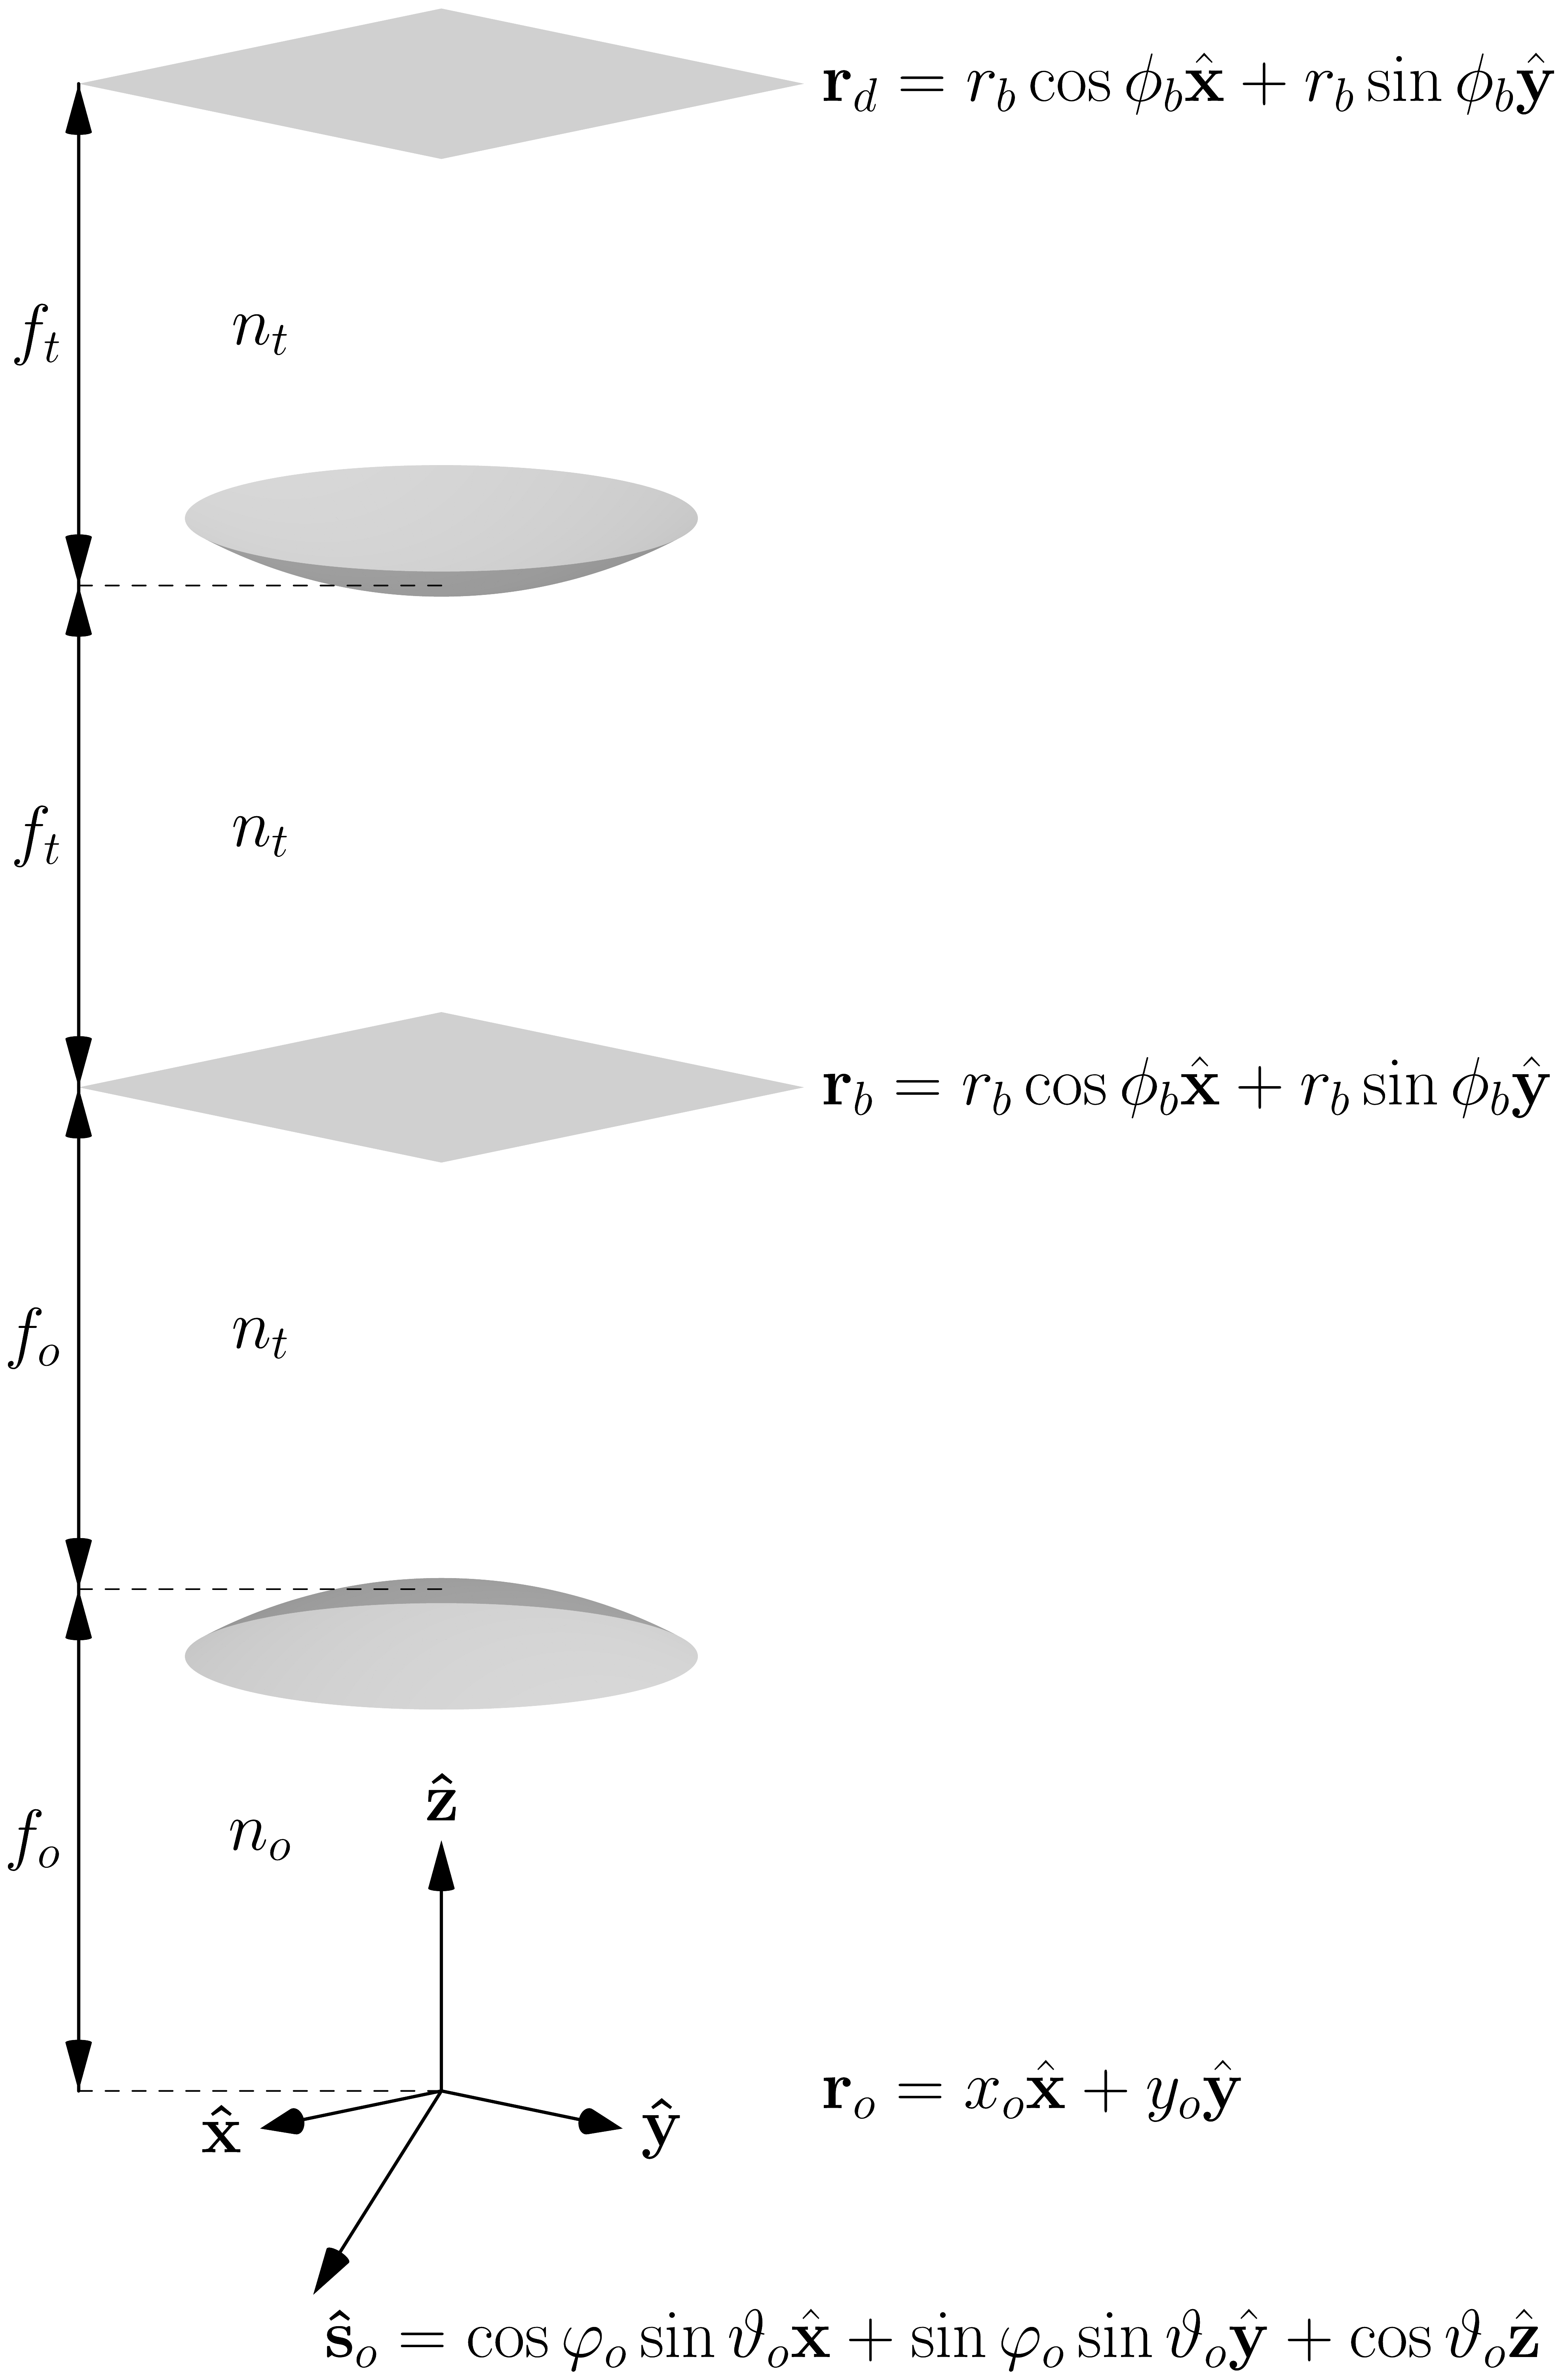
\includegraphics[width = 0.25\textwidth]{../figures/schematic.pdf}
   \caption{Simplified schematic of a single-view fluorescence microscope. The
     object is placed near the focal point of an objective lens with focal
     length $f_{o}$ in a medium with refractive index $n_o$. The object is
     parameterized by the 3D position vector $\ro{}$ ($\mb{o}$ for object) and a
     orientation unit vector $\so{}$. The light emitted by the fluorescent
     object is collected and collimated by the objective lens so that the
     electric fields are purely transverse in back focal plane. Points in the
     back focal plane are parameterized by a 2D position vector $\rb{}$
     ($\mb{b}$ for back focal plane). Finally, the tube lens with focal length
     $f_t$ refocuses the light onto a detector. Points on the detector are
     parameterized by a 2D position vector $\rd{}$ ($\mb{d}$ for detector). The
     back focal plane and detector are in a medium with refractive index
     $n_b$. Note that this schematic is not to scale---in typical microscopes
     $f_o \ll f_t$ to provide magnification.}
   \label{fig:frames_a}
\end{figure}

TODO: Show transverse shift invariance. 

TODO: Program up an efficient implementation of $h(\rd{}; \ro{}, \so{})$.

TODO: Plot select kernels.

\section{Spatio-angular Transfer Function}

TODO: Show angular band limit by taking angular Fourier transform only.

TODO: Show spatial band limit by taking the spatial Fourier transform of the
first angular term.

TODO: Evaluate and plot spatio-angular transfer function numerically. This
will be expensive, but it only has to be done once for each microscope. 

\section{Reconstruction}

\section{Conclusions}
\end{document}

